\documentclass[11pt,a4paper]{article}

% Packages
\usepackage[utf8]{inputenc}
\usepackage[T1]{fontenc}
\usepackage{geometry}
\usepackage{hyperref}
\usepackage{listings}
\usepackage{xcolor}
\usepackage{graphicx}
\usepackage{enumitem}
\usepackage{tcolorbox}
\usepackage{titlesec}
\usepackage{fancyhdr}
\usepackage{booktabs}
\usepackage{longtable}
\usepackage{tikz}

% Page geometry
\geometry{margin=1in}

% Colors
\definecolor{codebackground}{RGB}{245,245,245}
\definecolor{codeborder}{RGB}{200,200,200}
\definecolor{keyword}{RGB}{0,0,180}
\definecolor{string}{RGB}{0,128,0}
\definecolor{comment}{RGB}{128,128,128}
\definecolor{primary}{RGB}{59,130,246}
\definecolor{secondary}{RGB}{100,116,139}

% Code listing style
\lstdefinelanguage{TypeScript}{
  keywords={abstract, any, as, async, await, boolean, break, case, catch, class, const, constructor, continue, declare, default, delete, do, else, enum, export, extends, false, finally, for, from, function, get, if, implements, import, in, instanceof, interface, let, module, namespace, never, new, null, number, object, of, package, private, protected, public, readonly, require, return, set, static, string, super, switch, symbol, this, throw, true, try, type, typeof, undefined, unique, unknown, var, void, while, with, yield},
  sensitive=true,
  morecomment=[l]{//},
  morecomment=[s]{/*}{*/},
  morestring=[b]',
  morestring=[b]",
  morestring=[b]`
}

\lstset{
  language=TypeScript,
  backgroundcolor=\color{codebackground},
  basicstyle=\ttfamily\small,
  breaklines=true,
  captionpos=b,
  commentstyle=\color{comment},
  frame=single,
  framerule=0.5pt,
  rulecolor=\color{codeborder},
  keywordstyle=\color{keyword}\bfseries,
  stringstyle=\color{string},
  numbers=left,
  numberstyle=\tiny\color{secondary},
  numbersep=8pt,
  showstringspaces=false,
  tabsize=2,
  xleftmargin=15pt,
  framexleftmargin=15pt
}

% Header/Footer
\pagestyle{fancy}
\fancyhf{}
\fancyhead[L]{\textit{Chat Window/LLM Interface Specification}}
\fancyhead[R]{\textit{v1.0}}
\fancyfoot[C]{\thepage}

% Title formatting
\titleformat{\section}{\Large\bfseries\color{primary}}{\thesection}{1em}{}
\titleformat{\subsection}{\large\bfseries\color{secondary}}{\thesubsection}{1em}{}

% Custom boxes
\tcbuselibrary{skins,breakable}

\newtcolorbox{requirement}[1][]{
  colback=blue!5!white,
  colframe=primary,
  fonttitle=\bfseries,
  title=#1,
  breakable
}

\newtcolorbox{note}[1][Note]{
  colback=yellow!5!white,
  colframe=orange!75!black,
  fonttitle=\bfseries,
  title=#1,
  breakable
}

% Document info
\title{
  \vspace{-1cm}
  \textbf{Technical Specification}\\[0.5cm]
  \Large Chat Window / LLM Interface\\[0.3cm]
  \large Cursor-Style AI Assistant Integration
}
\author{Specification Document}
\date{January 2026 \\ Version 1.0}

\begin{document}

\maketitle
\thispagestyle{empty}

\vspace{1cm}

\begin{abstract}
This document provides a comprehensive technical specification for implementing a Cursor-style chat window and LLM interface within an existing TypeScript application. The chat window supports both local LLM inference (via Ollama or similar) and cloud API providers, features a collapsible panel positioned to the right of the Inspector panel, and provides context-aware AI assistance for development workflows.
\end{abstract}

\tableofcontents
\newpage

%==============================================================================
\section{Overview}
%==============================================================================

\subsection{Purpose}

This specification defines the architecture, interfaces, and implementation requirements for an integrated AI chat assistant panel. The system provides:

\begin{itemize}[noitemsep]
  \item Real-time conversational AI assistance within the application
  \item Context-aware responses utilizing application state and selected elements
  \item Support for multiple LLM backends (local and API-based)
  \item Streaming response rendering with code syntax highlighting
  \item Persistent conversation history with session management
\end{itemize}

\subsection{Scope}

The chat window component integrates into the existing application layout as a collapsible right-side panel adjacent to the Inspector panel. It operates independently while maintaining awareness of the application's current context.

\subsection{Design Goals}

\begin{enumerate}[noitemsep]
  \item \textbf{Stability}: Rock-solid operation with graceful degradation on failures
  \item \textbf{Performance}: Non-blocking UI with efficient streaming response handling
  \item \textbf{Flexibility}: Provider-agnostic LLM integration supporting local and cloud backends
  \item \textbf{Accessibility}: WCAG 2.1 AA compliance for all interactive elements
  \item \textbf{Developer Experience}: Clean TypeScript APIs with comprehensive type safety
\end{enumerate}

%==============================================================================
\section{Architecture}
%==============================================================================

\subsection{High-Level Component Diagram}

\begin{figure}[h]
\centering
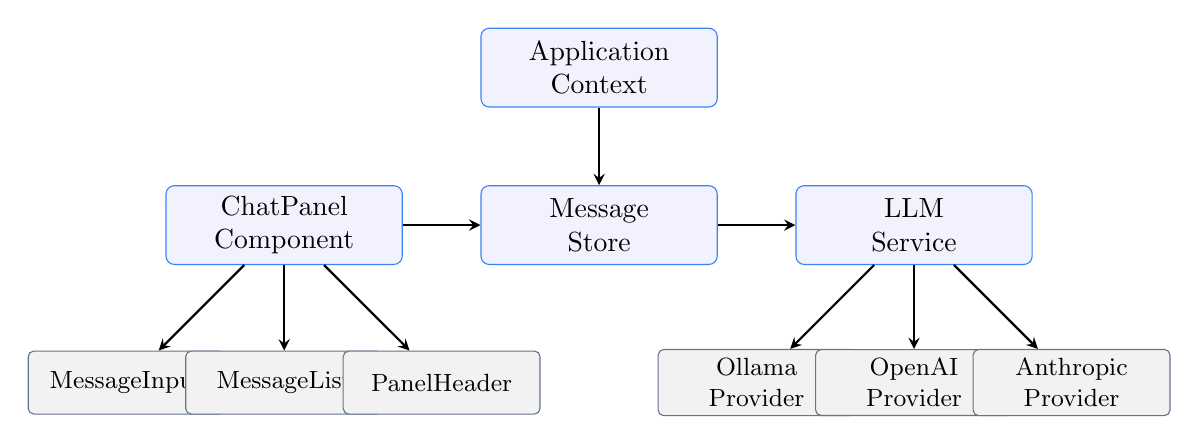
\begin{tikzpicture}[
  box/.style={rectangle, draw=primary, fill=blue!5, minimum width=3cm, minimum height=1cm, align=center, rounded corners=3pt},
  smallbox/.style={rectangle, draw=secondary, fill=gray!10, minimum width=2.5cm, minimum height=0.8cm, align=center, rounded corners=2pt, font=\small},
  arrow/.style={->, thick, >=stealth}
]

% Main components
\node[box] (chatpanel) at (0,0) {ChatPanel\\Component};
\node[box] (messagestore) at (4,0) {Message\\Store};
\node[box] (llmservice) at (8,0) {LLM\\Service};

% Sub-components
\node[smallbox] (input) at (-2,-2) {MessageInput};
\node[smallbox] (list) at (0,-2) {MessageList};
\node[smallbox] (header) at (2,-2) {PanelHeader};

% Providers
\node[smallbox] (ollama) at (6,-2) {Ollama\\Provider};
\node[smallbox] (openai) at (8,-2) {OpenAI\\Provider};
\node[smallbox] (anthropic) at (10,-2) {Anthropic\\Provider};

% Context
\node[box] (context) at (4,2) {Application\\Context};

% Arrows
\draw[arrow] (chatpanel) -- (messagestore);
\draw[arrow] (messagestore) -- (llmservice);
\draw[arrow] (context) -- (messagestore);

\draw[arrow] (chatpanel) -- (input);
\draw[arrow] (chatpanel) -- (list);
\draw[arrow] (chatpanel) -- (header);

\draw[arrow] (llmservice) -- (ollama);
\draw[arrow] (llmservice) -- (openai);
\draw[arrow] (llmservice) -- (anthropic);

\end{tikzpicture}
\caption{High-level architecture showing component relationships}
\end{figure}

\subsection{Module Structure}

\begin{lstlisting}
src/
  chat/
    components/
      ChatPanel.tsx           # Main panel container
      MessageList.tsx         # Scrollable message display
      MessageItem.tsx         # Individual message rendering
      MessageInput.tsx        # Input area with actions
      CodeBlock.tsx           # Syntax-highlighted code
      PanelHeader.tsx         # Title bar with controls
      ModelSelector.tsx       # LLM provider/model picker
      ContextIndicator.tsx    # Shows active context
    hooks/
      useChatStore.ts         # Zustand store hook
      useStreamingResponse.ts # SSE/streaming handler
      useLLMConnection.ts     # Provider connection state
      useAutoScroll.ts        # Smart scroll behavior
    services/
      LLMService.ts           # Provider abstraction layer
      providers/
        OllamaProvider.ts     # Local Ollama integration
        OpenAIProvider.ts     # OpenAI API provider
        AnthropicProvider.ts  # Anthropic API provider
        BaseProvider.ts       # Abstract base class
      ContextBuilder.ts       # Application context aggregator
      MessageFormatter.ts     # Markdown/code processing
    store/
      chatStore.ts            # Conversation state management
      settingsStore.ts        # User preferences
    types/
      index.ts                # Core type definitions
      messages.ts             # Message-related types
      providers.ts            # LLM provider types
      context.ts              # Application context types
    utils/
      tokenCounter.ts         # Token estimation utilities
      codeParser.ts           # Code block extraction
      streamParser.ts         # SSE stream parsing
    constants.ts              # Configuration constants
    index.ts                  # Public API exports
\end{lstlisting}

%==============================================================================
\section{TypeScript Type Definitions}
%==============================================================================

\subsection{Core Message Types}

\begin{lstlisting}
// types/messages.ts

export type MessageRole = 'user' | 'assistant' | 'system';

export type MessageStatus = 
  | 'pending'      // Awaiting send
  | 'streaming'    // Currently receiving
  | 'complete'     // Finished successfully
  | 'error'        // Failed with error
  | 'cancelled';   // User cancelled

export interface CodeBlock {
  readonly id: string;
  readonly language: string;
  readonly code: string;
  readonly startLine?: number;
  readonly filename?: string;
}

export interface MessageAttachment {
  readonly id: string;
  readonly type: 'file' | 'selection' | 'image' | 'context';
  readonly name: string;
  readonly content: string;
  readonly mimeType?: string;
  readonly metadata?: Record<string, unknown>;
}

export interface ChatMessage {
  readonly id: string;
  readonly role: MessageRole;
  readonly content: string;
  readonly timestamp: Date;
  readonly status: MessageStatus;
  readonly codeBlocks: readonly CodeBlock[];
  readonly attachments: readonly MessageAttachment[];
  readonly tokenCount?: number;
  readonly modelId?: string;
  readonly error?: ChatError;
  readonly metadata?: MessageMetadata;
}

export interface MessageMetadata {
  readonly duration?: number;        // Response time in ms
  readonly promptTokens?: number;
  readonly completionTokens?: number;
  readonly totalTokens?: number;
  readonly finishReason?: string;
}

export interface ChatError {
  readonly code: string;
  readonly message: string;
  readonly recoverable: boolean;
  readonly details?: unknown;
}

export interface Conversation {
  readonly id: string;
  readonly title: string;
  readonly messages: readonly ChatMessage[];
  readonly createdAt: Date;
  readonly updatedAt: Date;
  readonly modelId: string;
  readonly systemPrompt?: string;
  readonly contextConfig: ContextConfig;
}
\end{lstlisting}

\subsection{LLM Provider Types}

\begin{lstlisting}
// types/providers.ts

export type ProviderType = 'ollama' | 'openai' | 'anthropic' | 'custom';

export interface LLMModel {
  readonly id: string;
  readonly name: string;
  readonly provider: ProviderType;
  readonly contextWindow: number;
  readonly maxOutputTokens: number;
  readonly supportsStreaming: boolean;
  readonly supportsVision: boolean;
  readonly costPerInputToken?: number;
  readonly costPerOutputToken?: number;
}

export interface ProviderConfig {
  readonly type: ProviderType;
  readonly enabled: boolean;
  readonly baseUrl: string;
  readonly apiKey?: string;
  readonly defaultModel: string;
  readonly timeout: number;
  readonly maxRetries: number;
  readonly customHeaders?: Record<string, string>;
}

export interface OllamaConfig extends ProviderConfig {
  readonly type: 'ollama';
  readonly baseUrl: string;  // Default: http://localhost:11434
  readonly keepAlive?: string;
  readonly numGpu?: number;
  readonly numThread?: number;
}

export interface OpenAIConfig extends ProviderConfig {
  readonly type: 'openai';
  readonly apiKey: string;
  readonly organization?: string;
  readonly baseUrl: string;  // Default: https://api.openai.com/v1
}

export interface AnthropicConfig extends ProviderConfig {
  readonly type: 'anthropic';
  readonly apiKey: string;
  readonly baseUrl: string;  // Default: https://api.anthropic.com
  readonly apiVersion: string;
}

export type AnyProviderConfig = 
  | OllamaConfig 
  | OpenAIConfig 
  | AnthropicConfig;

export interface CompletionRequest {
  readonly messages: readonly ChatMessage[];
  readonly model: string;
  readonly temperature?: number;
  readonly maxTokens?: number;
  readonly topP?: number;
  readonly frequencyPenalty?: number;
  readonly presencePenalty?: number;
  readonly stop?: readonly string[];
  readonly stream?: boolean;
  readonly signal?: AbortSignal;
}

export interface CompletionResponse {
  readonly id: string;
  readonly content: string;
  readonly model: string;
  readonly finishReason: 'stop' | 'length' | 'error';
  readonly usage: TokenUsage;
}

export interface TokenUsage {
  readonly promptTokens: number;
  readonly completionTokens: number;
  readonly totalTokens: number;
}

export interface StreamChunk {
  readonly id: string;
  readonly delta: string;
  readonly finishReason?: string;
}

export type StreamCallback = (chunk: StreamChunk) => void;
export type ErrorCallback = (error: ChatError) => void;
\end{lstlisting}

\subsection{Application Context Types}

\begin{lstlisting}
// types/context.ts

export interface SelectionContext {
  readonly type: 'element' | 'text' | 'code' | 'range';
  readonly content: string;
  readonly elementIds?: readonly string[];
  readonly metadata?: Record<string, unknown>;
}

export interface FileContext {
  readonly path: string;
  readonly name: string;
  readonly content: string;
  readonly language?: string;
  readonly selection?: {
    readonly start: number;
    readonly end: number;
  };
}

export interface ApplicationContext {
  readonly selection: SelectionContext | null;
  readonly activeFile: FileContext | null;
  readonly openFiles: readonly FileContext[];
  readonly projectInfo: ProjectInfo | null;
  readonly customContext: Record<string, unknown>;
}

export interface ProjectInfo {
  readonly name: string;
  readonly type: string;
  readonly rootPath: string;
  readonly dependencies?: Record<string, string>;
}

export interface ContextConfig {
  readonly includeSelection: boolean;
  readonly includeActiveFile: boolean;
  readonly includeOpenFiles: boolean;
  readonly includeProjectInfo: boolean;
  readonly maxContextTokens: number;
  readonly customInstructions?: string;
}
\end{lstlisting}

\subsection{Store Types}

\begin{lstlisting}
// types/store.ts

export interface ChatState {
  // Conversations
  readonly conversations: Map<string, Conversation>;
  readonly activeConversationId: string | null;
  
  // UI State
  readonly isPanelOpen: boolean;
  readonly isPanelCollapsed: boolean;
  readonly isLoading: boolean;
  readonly error: ChatError | null;
  
  // Provider State
  readonly activeProvider: ProviderType;
  readonly activeModel: string;
  readonly providerStatus: Map<ProviderType, ProviderStatus>;
  
  // Context
  readonly contextConfig: ContextConfig;
  readonly applicationContext: ApplicationContext;
}

export interface ProviderStatus {
  readonly connected: boolean;
  readonly lastChecked: Date;
  readonly availableModels: readonly LLMModel[];
  readonly error?: string;
}

export interface ChatActions {
  // Panel
  togglePanel(): void;
  setCollapsed(collapsed: boolean): void;
  
  // Conversations
  createConversation(title?: string): string;
  deleteConversation(id: string): void;
  setActiveConversation(id: string): void;
  clearConversation(id: string): void;
  
  // Messages
  sendMessage(content: string, attachments?: MessageAttachment[]): Promise<void>;
  cancelStreaming(): void;
  retryMessage(messageId: string): Promise<void>;
  deleteMessage(messageId: string): void;
  
  // Provider
  setProvider(provider: ProviderType): void;
  setModel(modelId: string): void;
  refreshProviderStatus(provider: ProviderType): Promise<void>;
  
  // Context
  updateContextConfig(config: Partial<ContextConfig>): void;
  refreshApplicationContext(): void;
}

export type ChatStore = ChatState & ChatActions;
\end{lstlisting}

%==============================================================================
\section{LLM Service Implementation}
%==============================================================================

\subsection{Abstract Provider Base}

\begin{lstlisting}
// services/providers/BaseProvider.ts

export abstract class BaseProvider {
  protected config: ProviderConfig;
  protected abortController: AbortController | null = null;

  constructor(config: ProviderConfig) {
    this.config = config;
  }

  abstract get name(): string;
  abstract get type(): ProviderType;
  
  abstract connect(): Promise<boolean>;
  abstract disconnect(): Promise<void>;
  abstract isConnected(): boolean;
  
  abstract listModels(): Promise<LLMModel[]>;
  
  abstract complete(
    request: CompletionRequest
  ): Promise<CompletionResponse>;
  
  abstract stream(
    request: CompletionRequest,
    onChunk: StreamCallback,
    onError: ErrorCallback
  ): Promise<void>;

  cancel(): void {
    if (this.abortController) {
      this.abortController.abort();
      this.abortController = null;
    }
  }

  protected createAbortController(): AbortController {
    this.cancel();
    this.abortController = new AbortController();
    return this.abortController;
  }

  protected async fetchWithRetry(
    url: string,
    options: RequestInit,
    retries = this.config.maxRetries
  ): Promise<Response> {
    let lastError: Error | null = null;
    
    for (let i = 0; i <= retries; i++) {
      try {
        const response = await fetch(url, {
          ...options,
          signal: this.abortController?.signal,
        });
        
        if (response.ok) return response;
        
        if (response.status >= 500 && i < retries) {
          await this.delay(Math.pow(2, i) * 1000);
          continue;
        }
        
        throw new Error(`HTTP ${response.status}: ${response.statusText}`);
      } catch (error) {
        lastError = error as Error;
        if (error instanceof Error && error.name === 'AbortError') {
          throw error;
        }
        if (i < retries) {
          await this.delay(Math.pow(2, i) * 1000);
        }
      }
    }
    
    throw lastError;
  }

  private delay(ms: number): Promise<void> {
    return new Promise(resolve => setTimeout(resolve, ms));
  }
}
\end{lstlisting}

\subsection{Ollama Provider Implementation}

\begin{lstlisting}
// services/providers/OllamaProvider.ts

import { BaseProvider } from './BaseProvider';

export class OllamaProvider extends BaseProvider {
  private connected = false;

  get name(): string { return 'Ollama'; }
  get type(): ProviderType { return 'ollama'; }

  async connect(): Promise<boolean> {
    try {
      const response = await fetch(`${this.config.baseUrl}/api/tags`);
      this.connected = response.ok;
      return this.connected;
    } catch {
      this.connected = false;
      return false;
    }
  }

  async disconnect(): Promise<void> {
    this.connected = false;
  }

  isConnected(): boolean {
    return this.connected;
  }

  async listModels(): Promise<LLMModel[]> {
    const response = await this.fetchWithRetry(
      `${this.config.baseUrl}/api/tags`,
      { method: 'GET' }
    );
    
    const data = await response.json();
    
    return data.models.map((model: any) => ({
      id: model.name,
      name: model.name,
      provider: 'ollama',
      contextWindow: model.details?.parameter_size || 4096,
      maxOutputTokens: 4096,
      supportsStreaming: true,
      supportsVision: model.details?.families?.includes('clip') ?? false,
    }));
  }

  async complete(request: CompletionRequest): Promise<CompletionResponse> {
    const controller = this.createAbortController();
    
    const response = await this.fetchWithRetry(
      `${this.config.baseUrl}/api/chat`,
      {
        method: 'POST',
        headers: { 'Content-Type': 'application/json' },
        body: JSON.stringify({
          model: request.model,
          messages: this.formatMessages(request.messages),
          stream: false,
          options: {
            temperature: request.temperature ?? 0.7,
            num_predict: request.maxTokens ?? 2048,
            top_p: request.topP ?? 0.9,
            stop: request.stop,
          },
        }),
        signal: controller.signal,
      }
    );

    const data = await response.json();

    return {
      id: crypto.randomUUID(),
      content: data.message.content,
      model: request.model,
      finishReason: data.done ? 'stop' : 'length',
      usage: {
        promptTokens: data.prompt_eval_count ?? 0,
        completionTokens: data.eval_count ?? 0,
        totalTokens: (data.prompt_eval_count ?? 0) + (data.eval_count ?? 0),
      },
    };
  }

  async stream(
    request: CompletionRequest,
    onChunk: StreamCallback,
    onError: ErrorCallback
  ): Promise<void> {
    const controller = this.createAbortController();
    
    try {
      const response = await fetch(`${this.config.baseUrl}/api/chat`, {
        method: 'POST',
        headers: { 'Content-Type': 'application/json' },
        body: JSON.stringify({
          model: request.model,
          messages: this.formatMessages(request.messages),
          stream: true,
          options: {
            temperature: request.temperature ?? 0.7,
            num_predict: request.maxTokens ?? 2048,
            top_p: request.topP ?? 0.9,
            stop: request.stop,
          },
        }),
        signal: controller.signal,
      });

      if (!response.ok) {
        throw new Error(`HTTP ${response.status}`);
      }

      const reader = response.body?.getReader();
      if (!reader) throw new Error('No response body');

      const decoder = new TextDecoder();
      let buffer = '';

      while (true) {
        const { done, value } = await reader.read();
        if (done) break;

        buffer += decoder.decode(value, { stream: true });
        const lines = buffer.split('\n');
        buffer = lines.pop() ?? '';

        for (const line of lines) {
          if (!line.trim()) continue;
          
          try {
            const data = JSON.parse(line);
            onChunk({
              id: crypto.randomUUID(),
              delta: data.message?.content ?? '',
              finishReason: data.done ? 'stop' : undefined,
            });
          } catch (e) {
            // Skip malformed JSON
          }
        }
      }
    } catch (error) {
      if (error instanceof Error && error.name !== 'AbortError') {
        onError({
          code: 'STREAM_ERROR',
          message: error.message,
          recoverable: true,
        });
      }
    }
  }

  private formatMessages(messages: readonly ChatMessage[]): any[] {
    return messages.map(msg => ({
      role: msg.role,
      content: msg.content,
    }));
  }
}
\end{lstlisting}

\subsection{LLM Service Facade}

\begin{lstlisting}
// services/LLMService.ts

import { OllamaProvider } from './providers/OllamaProvider';
import { OpenAIProvider } from './providers/OpenAIProvider';
import { AnthropicProvider } from './providers/AnthropicProvider';

export class LLMService {
  private providers: Map<ProviderType, BaseProvider> = new Map();
  private activeProvider: BaseProvider | null = null;

  constructor(configs: AnyProviderConfig[]) {
    for (const config of configs) {
      if (!config.enabled) continue;
      
      const provider = this.createProvider(config);
      if (provider) {
        this.providers.set(config.type, provider);
      }
    }
  }

  private createProvider(config: AnyProviderConfig): BaseProvider | null {
    switch (config.type) {
      case 'ollama':
        return new OllamaProvider(config);
      case 'openai':
        return new OpenAIProvider(config);
      case 'anthropic':
        return new AnthropicProvider(config);
      default:
        return null;
    }
  }

  async initialize(): Promise<Map<ProviderType, boolean>> {
    const results = new Map<ProviderType, boolean>();
    
    for (const [type, provider] of this.providers) {
      const connected = await provider.connect();
      results.set(type, connected);
    }
    
    // Set first connected provider as active
    for (const [type, connected] of results) {
      if (connected) {
        this.activeProvider = this.providers.get(type) ?? null;
        break;
      }
    }
    
    return results;
  }

  setActiveProvider(type: ProviderType): boolean {
    const provider = this.providers.get(type);
    if (provider?.isConnected()) {
      this.activeProvider = provider;
      return true;
    }
    return false;
  }

  getActiveProvider(): BaseProvider | null {
    return this.activeProvider;
  }

  async complete(request: CompletionRequest): Promise<CompletionResponse> {
    if (!this.activeProvider) {
      throw new Error('No active LLM provider');
    }
    return this.activeProvider.complete(request);
  }

  async stream(
    request: CompletionRequest,
    onChunk: StreamCallback,
    onError: ErrorCallback
  ): Promise<void> {
    if (!this.activeProvider) {
      throw new Error('No active LLM provider');
    }
    return this.activeProvider.stream(request, onChunk, onError);
  }

  cancel(): void {
    this.activeProvider?.cancel();
  }

  async listModels(type?: ProviderType): Promise<LLMModel[]> {
    if (type) {
      const provider = this.providers.get(type);
      return provider?.listModels() ?? [];
    }
    
    const allModels: LLMModel[] = [];
    for (const provider of this.providers.values()) {
      if (provider.isConnected()) {
        allModels.push(...await provider.listModels());
      }
    }
    return allModels;
  }
}
\end{lstlisting}

%==============================================================================
\section{UI Component Specifications}
%==============================================================================

\subsection{Panel Layout}

\begin{requirement}[Layout Requirements]
\begin{itemize}[noitemsep]
  \item Position: Right side of application, adjacent to Inspector panel
  \item Default width: 400px (configurable: 300px--600px)
  \item Collapsible: Minimize to 48px icon strip
  \item Resizable: Horizontal drag handle on left edge
  \item Z-index: Above main canvas, below modals (z-index: 100)
  \item Responsive: Collapse automatically below 1200px viewport width
\end{itemize}
\end{requirement}

\begin{lstlisting}
// components/ChatPanel.tsx

import { useState, useCallback, useRef } from 'react';
import { useChatStore } from '../hooks/useChatStore';

interface ChatPanelProps {
  defaultWidth?: number;
  minWidth?: number;
  maxWidth?: number;
  collapsedWidth?: number;
}

export const ChatPanel: React.FC<ChatPanelProps> = ({
  defaultWidth = 400,
  minWidth = 300,
  maxWidth = 600,
  collapsedWidth = 48,
}) => {
  const {
    isPanelOpen,
    isPanelCollapsed,
    isLoading,
    togglePanel,
    setCollapsed,
  } = useChatStore();

  const [width, setWidth] = useState(defaultWidth);
  const panelRef = useRef<HTMLDivElement>(null);
  const resizing = useRef(false);

  const handleResizeStart = useCallback((e: React.MouseEvent) => {
    e.preventDefault();
    resizing.current = true;
    
    const startX = e.clientX;
    const startWidth = width;

    const handleMouseMove = (e: MouseEvent) => {
      if (!resizing.current) return;
      const delta = startX - e.clientX;
      const newWidth = Math.min(maxWidth, Math.max(minWidth, startWidth + delta));
      setWidth(newWidth);
    };

    const handleMouseUp = () => {
      resizing.current = false;
      document.removeEventListener('mousemove', handleMouseMove);
      document.removeEventListener('mouseup', handleMouseUp);
    };

    document.addEventListener('mousemove', handleMouseMove);
    document.addEventListener('mouseup', handleMouseUp);
  }, [width, minWidth, maxWidth]);

  if (!isPanelOpen) return null;

  const panelWidth = isPanelCollapsed ? collapsedWidth : width;

  return (
    <aside
      ref={panelRef}
      className="chat-panel"
      style={{ width: panelWidth }}
      aria-label="AI Chat Assistant"
      role="complementary"
    >
      {/* Resize Handle */}
      {!isPanelCollapsed && (
        <div
          className="chat-panel__resize-handle"
          onMouseDown={handleResizeStart}
          role="separator"
          aria-orientation="vertical"
          aria-label="Resize chat panel"
        />
      )}

      {/* Panel Content */}
      {isPanelCollapsed ? (
        <CollapsedPanel onExpand={() => setCollapsed(false)} />
      ) : (
        <>
          <PanelHeader onCollapse={() => setCollapsed(true)} />
          <MessageList />
          <MessageInput disabled={isLoading} />
        </>
      )}
    </aside>
  );
};
\end{lstlisting}

\subsection{Message List Component}

\begin{lstlisting}
// components/MessageList.tsx

import { useRef, useEffect, useCallback } from 'react';
import { useChatStore } from '../hooks/useChatStore';
import { useAutoScroll } from '../hooks/useAutoScroll';
import { MessageItem } from './MessageItem';

export const MessageList: React.FC = () => {
  const { activeConversation } = useChatStore();
  const containerRef = useRef<HTMLDivElement>(null);
  const { scrollToBottom, isAtBottom } = useAutoScroll(containerRef);

  const messages = activeConversation?.messages ?? [];

  // Auto-scroll on new messages when at bottom
  useEffect(() => {
    if (isAtBottom) {
      scrollToBottom();
    }
  }, [messages.length, isAtBottom, scrollToBottom]);

  if (messages.length === 0) {
    return (
      <div className="message-list message-list--empty">
        <div className="message-list__placeholder">
          <IconSparkles size={48} />
          <h3>Start a conversation</h3>
          <p>Ask questions, get help with code, or discuss your project.</p>
        </div>
      </div>
    );
  }

  return (
    <div
      ref={containerRef}
      className="message-list"
      role="log"
      aria-live="polite"
      aria-label="Conversation messages"
    >
      {messages.map((message, index) => (
        <MessageItem
          key={message.id}
          message={message}
          isLast={index === messages.length - 1}
        />
      ))}
    </div>
  );
};
\end{lstlisting}

\subsection{Message Input Component}

\begin{lstlisting}
// components/MessageInput.tsx

import { useState, useRef, useCallback, KeyboardEvent } from 'react';
import { useChatStore } from '../hooks/useChatStore';

interface MessageInputProps {
  disabled?: boolean;
  maxLength?: number;
}

export const MessageInput: React.FC<MessageInputProps> = ({
  disabled = false,
  maxLength = 32000,
}) => {
  const [input, setInput] = useState('');
  const [attachments, setAttachments] = useState<MessageAttachment[]>([]);
  const textareaRef = useRef<HTMLTextAreaElement>(null);
  
  const { sendMessage, isLoading, cancelStreaming } = useChatStore();

  const handleSubmit = useCallback(async () => {
    const trimmed = input.trim();
    if (!trimmed || disabled || isLoading) return;

    setInput('');
    setAttachments([]);
    
    await sendMessage(trimmed, attachments);
  }, [input, attachments, disabled, isLoading, sendMessage]);

  const handleKeyDown = useCallback((e: KeyboardEvent<HTMLTextAreaElement>) => {
    if (e.key === 'Enter' && !e.shiftKey) {
      e.preventDefault();
      handleSubmit();
    }
  }, [handleSubmit]);

  // Auto-resize textarea
  useEffect(() => {
    const textarea = textareaRef.current;
    if (textarea) {
      textarea.style.height = 'auto';
      textarea.style.height = `${Math.min(textarea.scrollHeight, 200)}px`;
    }
  }, [input]);

  return (
    <div className="message-input">
      {/* Attachments Preview */}
      {attachments.length > 0 && (
        <AttachmentList
          attachments={attachments}
          onRemove={(id) => setAttachments(a => a.filter(x => x.id !== id))}
        />
      )}

      {/* Input Area */}
      <div className="message-input__field">
        <textarea
          ref={textareaRef}
          value={input}
          onChange={(e) => setInput(e.target.value)}
          onKeyDown={handleKeyDown}
          placeholder="Ask anything..."
          disabled={disabled}
          maxLength={maxLength}
          rows={1}
          aria-label="Message input"
        />

        {/* Actions */}
        <div className="message-input__actions">
          <AttachButton onAttach={(a) => setAttachments(prev => [...prev, a])} />
          
          {isLoading ? (
            <button
              onClick={cancelStreaming}
              className="message-input__cancel"
              aria-label="Cancel response"
            >
              <IconStop size={20} />
            </button>
          ) : (
            <button
              onClick={handleSubmit}
              disabled={!input.trim() || disabled}
              className="message-input__send"
              aria-label="Send message"
            >
              <IconSend size={20} />
            </button>
          )}
        </div>
      </div>

      {/* Character Count */}
      <div className="message-input__footer">
        <span className="message-input__count">
          {input.length} / {maxLength}
        </span>
        <ModelIndicator />
      </div>
    </div>
  );
};
\end{lstlisting}

\subsection{Code Block Rendering}

\begin{lstlisting}
// components/CodeBlock.tsx

import { useState, useCallback } from 'react';
import { highlight, languages } from 'prismjs';
import 'prismjs/components/prism-typescript';
import 'prismjs/components/prism-javascript';
import 'prismjs/components/prism-python';
import 'prismjs/components/prism-css';
import 'prismjs/components/prism-json';

interface CodeBlockProps {
  code: string;
  language: string;
  filename?: string;
  showLineNumbers?: boolean;
  onCopy?: () => void;
  onInsert?: (code: string) => void;
}

export const CodeBlock: React.FC<CodeBlockProps> = ({
  code,
  language,
  filename,
  showLineNumbers = true,
  onCopy,
  onInsert,
}) => {
  const [copied, setCopied] = useState(false);

  const handleCopy = useCallback(async () => {
    await navigator.clipboard.writeText(code);
    setCopied(true);
    onCopy?.();
    setTimeout(() => setCopied(false), 2000);
  }, [code, onCopy]);

  const highlightedCode = highlight(
    code,
    languages[language] || languages.plaintext,
    language
  );

  return (
    <div className="code-block">
      {/* Header */}
      <div className="code-block__header">
        {filename && (
          <span className="code-block__filename">
            <IconFile size={14} />
            {filename}
          </span>
        )}
        <span className="code-block__language">{language}</span>
        
        <div className="code-block__actions">
          {onInsert && (
            <button
              onClick={() => onInsert(code)}
              className="code-block__action"
              title="Insert at cursor"
            >
              <IconCursorText size={16} />
            </button>
          )}
          <button
            onClick={handleCopy}
            className="code-block__action"
            title={copied ? 'Copied!' : 'Copy code'}
          >
            {copied ? <IconCheck size={16} /> : <IconCopy size={16} />}
          </button>
        </div>
      </div>

      {/* Code Content */}
      <pre className="code-block__content">
        <code
          className={`language-${language}`}
          dangerouslySetInnerHTML={{ __html: highlightedCode }}
        />
      </pre>
    </div>
  );
};
\end{lstlisting}

%==============================================================================
\section{State Management}
%==============================================================================

\subsection{Zustand Store Implementation}

\begin{lstlisting}
// store/chatStore.ts

import { create } from 'zustand';
import { devtools, persist } from 'zustand/middleware';
import { immer } from 'zustand/middleware/immer';

export const useChatStore = create<ChatStore>()(
  devtools(
    persist(
      immer((set, get) => ({
        // Initial State
        conversations: new Map(),
        activeConversationId: null,
        isPanelOpen: false,
        isPanelCollapsed: false,
        isLoading: false,
        error: null,
        activeProvider: 'ollama',
        activeModel: 'llama3.1:8b',
        providerStatus: new Map(),
        contextConfig: {
          includeSelection: true,
          includeActiveFile: true,
          includeOpenFiles: false,
          includeProjectInfo: true,
          maxContextTokens: 8000,
        },
        applicationContext: {
          selection: null,
          activeFile: null,
          openFiles: [],
          projectInfo: null,
          customContext: {},
        },

        // Panel Actions
        togglePanel: () => set(state => {
          state.isPanelOpen = !state.isPanelOpen;
        }),

        setCollapsed: (collapsed) => set(state => {
          state.isPanelCollapsed = collapsed;
        }),

        // Conversation Actions
        createConversation: (title) => {
          const id = crypto.randomUUID();
          const conversation: Conversation = {
            id,
            title: title ?? `Chat ${new Date().toLocaleDateString()}`,
            messages: [],
            createdAt: new Date(),
            updatedAt: new Date(),
            modelId: get().activeModel,
            contextConfig: get().contextConfig,
          };
          
          set(state => {
            state.conversations.set(id, conversation);
            state.activeConversationId = id;
          });
          
          return id;
        },

        deleteConversation: (id) => set(state => {
          state.conversations.delete(id);
          if (state.activeConversationId === id) {
            const remaining = Array.from(state.conversations.keys());
            state.activeConversationId = remaining[0] ?? null;
          }
        }),

        setActiveConversation: (id) => set(state => {
          if (state.conversations.has(id)) {
            state.activeConversationId = id;
          }
        }),

        clearConversation: (id) => set(state => {
          const conv = state.conversations.get(id);
          if (conv) {
            conv.messages = [];
            conv.updatedAt = new Date();
          }
        }),

        // Message Actions
        sendMessage: async (content, attachments = []) => {
          const { activeConversationId, activeModel } = get();
          
          let conversationId = activeConversationId;
          if (!conversationId) {
            conversationId = get().createConversation();
          }

          // Create user message
          const userMessage: ChatMessage = {
            id: crypto.randomUUID(),
            role: 'user',
            content,
            timestamp: new Date(),
            status: 'complete',
            codeBlocks: [],
            attachments,
          };

          // Create placeholder assistant message
          const assistantMessage: ChatMessage = {
            id: crypto.randomUUID(),
            role: 'assistant',
            content: '',
            timestamp: new Date(),
            status: 'streaming',
            codeBlocks: [],
            attachments: [],
            modelId: activeModel,
          };

          // Add messages to conversation
          set(state => {
            const conv = state.conversations.get(conversationId!);
            if (conv) {
              conv.messages = [...conv.messages, userMessage, assistantMessage];
              conv.updatedAt = new Date();
            }
            state.isLoading = true;
            state.error = null;
          });

          // Stream response
          try {
            const llmService = getLLMService();
            const conv = get().conversations.get(conversationId);
            
            await llmService.stream(
              {
                messages: conv?.messages ?? [],
                model: activeModel,
                temperature: 0.7,
                maxTokens: 4096,
              },
              // On chunk
              (chunk) => {
                set(state => {
                  const conv = state.conversations.get(conversationId!);
                  if (conv) {
                    const msgIndex = conv.messages.findIndex(
                      m => m.id === assistantMessage.id
                    );
                    if (msgIndex >= 0) {
                      const msg = conv.messages[msgIndex];
                      conv.messages[msgIndex] = {
                        ...msg,
                        content: msg.content + chunk.delta,
                        status: chunk.finishReason ? 'complete' : 'streaming',
                      };
                    }
                  }
                });
              },
              // On error
              (error) => {
                set(state => {
                  state.error = error;
                  const conv = state.conversations.get(conversationId!);
                  if (conv) {
                    const msgIndex = conv.messages.findIndex(
                      m => m.id === assistantMessage.id
                    );
                    if (msgIndex >= 0) {
                      conv.messages[msgIndex] = {
                        ...conv.messages[msgIndex],
                        status: 'error',
                        error,
                      };
                    }
                  }
                });
              }
            );
          } finally {
            set(state => {
              state.isLoading = false;
            });
          }
        },

        cancelStreaming: () => {
          getLLMService().cancel();
          set(state => {
            state.isLoading = false;
            const convId = state.activeConversationId;
            if (convId) {
              const conv = state.conversations.get(convId);
              if (conv) {
                const lastMsg = conv.messages[conv.messages.length - 1];
                if (lastMsg?.status === 'streaming') {
                  conv.messages[conv.messages.length - 1] = {
                    ...lastMsg,
                    status: 'cancelled',
                  };
                }
              }
            }
          });
        },

        retryMessage: async (messageId) => {
          // Implementation for retry logic
        },

        deleteMessage: (messageId) => set(state => {
          const convId = state.activeConversationId;
          if (convId) {
            const conv = state.conversations.get(convId);
            if (conv) {
              conv.messages = conv.messages.filter(m => m.id !== messageId);
            }
          }
        }),

        // Provider Actions
        setProvider: (provider) => set(state => {
          state.activeProvider = provider;
        }),

        setModel: (modelId) => set(state => {
          state.activeModel = modelId;
        }),

        refreshProviderStatus: async (provider) => {
          // Implementation for provider status refresh
        },

        // Context Actions
        updateContextConfig: (config) => set(state => {
          state.contextConfig = { ...state.contextConfig, ...config };
        }),

        refreshApplicationContext: () => {
          // Hook into application state to get current context
        },
      })),
      {
        name: 'chat-storage',
        partialize: (state) => ({
          conversations: Array.from(state.conversations.entries()),
          activeProvider: state.activeProvider,
          activeModel: state.activeModel,
          contextConfig: state.contextConfig,
        }),
      }
    ),
    { name: 'ChatStore' }
  )
);
\end{lstlisting}

%==============================================================================
\section{Context Building}
%==============================================================================

\subsection{Context Builder Service}

\begin{lstlisting}
// services/ContextBuilder.ts

export class ContextBuilder {
  private config: ContextConfig;
  private tokenCounter: TokenCounter;

  constructor(config: ContextConfig) {
    this.config = config;
    this.tokenCounter = new TokenCounter();
  }

  build(context: ApplicationContext): string {
    const sections: string[] = [];
    let totalTokens = 0;

    // System instructions
    const systemPrompt = this.buildSystemPrompt();
    sections.push(systemPrompt);
    totalTokens += this.tokenCounter.count(systemPrompt);

    // Selection context
    if (this.config.includeSelection && context.selection) {
      const selectionCtx = this.formatSelection(context.selection);
      const tokens = this.tokenCounter.count(selectionCtx);
      
      if (totalTokens + tokens <= this.config.maxContextTokens) {
        sections.push(selectionCtx);
        totalTokens += tokens;
      }
    }

    // Active file context
    if (this.config.includeActiveFile && context.activeFile) {
      const fileCtx = this.formatFile(context.activeFile);
      const tokens = this.tokenCounter.count(fileCtx);
      
      if (totalTokens + tokens <= this.config.maxContextTokens) {
        sections.push(fileCtx);
        totalTokens += tokens;
      }
    }

    // Project info
    if (this.config.includeProjectInfo && context.projectInfo) {
      const projectCtx = this.formatProject(context.projectInfo);
      const tokens = this.tokenCounter.count(projectCtx);
      
      if (totalTokens + tokens <= this.config.maxContextTokens) {
        sections.push(projectCtx);
        totalTokens += tokens;
      }
    }

    // Custom instructions
    if (this.config.customInstructions) {
      sections.push(`\n## Custom Instructions\n${this.config.customInstructions}`);
    }

    return sections.join('\n\n');
  }

  private buildSystemPrompt(): string {
    return `You are an AI assistant integrated into a design/development application.
Your role is to help users with:
- Understanding and modifying their designs
- Writing and debugging code
- Explaining concepts and best practices
- Answering questions about the application

Always be concise and helpful. When providing code, use appropriate syntax highlighting.
If you're unsure about something, ask for clarification.`;
  }

  private formatSelection(selection: SelectionContext): string {
    return `## Current Selection
Type: ${selection.type}
${selection.elementIds ? `Elements: ${selection.elementIds.join(', ')}` : ''}

\`\`\`
${selection.content}
\`\`\``;
  }

  private formatFile(file: FileContext): string {
    const lang = file.language ?? this.detectLanguage(file.name);
    let content = file.content;

    // Highlight selection if present
    if (file.selection) {
      content = this.highlightSelection(content, file.selection);
    }

    return `## Active File: ${file.name}
Path: ${file.path}

\`\`\`${lang}
${content}
\`\`\``;
  }

  private formatProject(project: ProjectInfo): string {
    return `## Project Information
Name: ${project.name}
Type: ${project.type}
Path: ${project.rootPath}`;
  }

  private detectLanguage(filename: string): string {
    const ext = filename.split('.').pop()?.toLowerCase();
    const langMap: Record<string, string> = {
      ts: 'typescript',
      tsx: 'typescript',
      js: 'javascript',
      jsx: 'javascript',
      py: 'python',
      css: 'css',
      json: 'json',
      html: 'html',
    };
    return langMap[ext ?? ''] ?? 'plaintext';
  }

  private highlightSelection(
    content: string,
    selection: { start: number; end: number }
  ): string {
    const before = content.slice(0, selection.start);
    const selected = content.slice(selection.start, selection.end);
    const after = content.slice(selection.end);
    return `${before}/* >>> SELECTED START >>> */${selected}/* <<< SELECTED END <<< */${after}`;
  }
}
\end{lstlisting}

%==============================================================================
\section{Configuration}
%==============================================================================

\subsection{Default Configuration}

\begin{lstlisting}
// constants.ts

export const DEFAULT_PROVIDERS: AnyProviderConfig[] = [
  {
    type: 'ollama',
    enabled: true,
    baseUrl: 'http://localhost:11434',
    defaultModel: 'llama3.1:8b',
    timeout: 120000,
    maxRetries: 3,
  },
  {
    type: 'openai',
    enabled: false,
    baseUrl: 'https://api.openai.com/v1',
    apiKey: '',
    defaultModel: 'gpt-4-turbo',
    timeout: 60000,
    maxRetries: 3,
  },
  {
    type: 'anthropic',
    enabled: false,
    baseUrl: 'https://api.anthropic.com',
    apiKey: '',
    apiVersion: '2024-01-01',
    defaultModel: 'claude-3-sonnet-20240229',
    timeout: 60000,
    maxRetries: 3,
  },
];

export const PANEL_CONFIG = {
  defaultWidth: 400,
  minWidth: 300,
  maxWidth: 600,
  collapsedWidth: 48,
  autoCollapseBreakpoint: 1200,
} as const;

export const MESSAGE_CONFIG = {
  maxLength: 32000,
  maxAttachments: 10,
  maxAttachmentSize: 10 * 1024 * 1024, // 10MB
} as const;

export const CONTEXT_CONFIG: ContextConfig = {
  includeSelection: true,
  includeActiveFile: true,
  includeOpenFiles: false,
  includeProjectInfo: true,
  maxContextTokens: 8000,
};

export const SUPPORTED_CODE_LANGUAGES = [
  'typescript',
  'javascript',
  'python',
  'css',
  'html',
  'json',
  'markdown',
  'yaml',
  'sql',
  'bash',
  'rust',
  'go',
] as const;
\end{lstlisting}

%==============================================================================
\section{Accessibility Requirements}
%==============================================================================

\subsection{WCAG 2.1 AA Compliance}

\begin{requirement}[Accessibility Requirements]
\begin{enumerate}[noitemsep]
  \item \textbf{Keyboard Navigation}:
    \begin{itemize}[noitemsep]
      \item All interactive elements focusable via Tab
      \item Escape closes panel/cancels streaming
      \item Enter sends message (Shift+Enter for newline)
      \item Arrow keys navigate conversation history
    \end{itemize}
  
  \item \textbf{Screen Reader Support}:
    \begin{itemize}[noitemsep]
      \item ARIA labels on all interactive elements
      \item Live regions for streaming responses
      \item Proper heading hierarchy
      \item Descriptive button labels
    \end{itemize}
  
  \item \textbf{Visual Accessibility}:
    \begin{itemize}[noitemsep]
      \item Minimum contrast ratio 4.5:1 for text
      \item Focus indicators visible (2px outline minimum)
      \item No reliance on color alone for information
      \item Resizable text up to 200\%
    \end{itemize}
  
  \item \textbf{Motion/Animation}:
    \begin{itemize}[noitemsep]
      \item Respect \texttt{prefers-reduced-motion}
      \item No auto-playing animations
      \item Typing indicator can be disabled
    \end{itemize}
\end{enumerate}
\end{requirement}

%==============================================================================
\section{Error Handling}
%==============================================================================

\subsection{Error Categories and Recovery}

\begin{longtable}{@{}llp{6cm}@{}}
\toprule
\textbf{Error Code} & \textbf{Category} & \textbf{Recovery Strategy} \\
\midrule
\endhead
\texttt{PROVIDER\_OFFLINE} & Connection & Auto-retry with exponential backoff; fallback to alternative provider \\
\texttt{RATE\_LIMITED} & API & Queue requests; display cooldown timer \\
\texttt{CONTEXT\_TOO\_LARGE} & Input & Truncate context; warn user \\
\texttt{MODEL\_NOT\_FOUND} & Configuration & Fallback to default model; prompt reconfiguration \\
\texttt{STREAM\_INTERRUPTED} & Network & Offer retry; preserve partial response \\
\texttt{AUTH\_FAILED} & API & Prompt for credential update \\
\texttt{TIMEOUT} & Network & Cancel request; offer retry \\
\texttt{INVALID\_RESPONSE} & API & Log error; display generic message \\
\bottomrule
\end{longtable}

\begin{lstlisting}
// utils/errorHandler.ts

export function handleChatError(error: ChatError): ErrorRecovery {
  const strategies: Record<string, ErrorRecovery> = {
    PROVIDER_OFFLINE: {
      action: 'retry',
      message: 'Connection lost. Retrying...',
      retryDelay: 2000,
      maxRetries: 3,
      fallback: () => tryAlternativeProvider(),
    },
    RATE_LIMITED: {
      action: 'wait',
      message: 'Rate limited. Please wait...',
      retryDelay: 60000,
      maxRetries: 1,
    },
    CONTEXT_TOO_LARGE: {
      action: 'modify',
      message: 'Context too large. Reducing...',
      modification: () => truncateContext(),
    },
    STREAM_INTERRUPTED: {
      action: 'prompt',
      message: 'Response interrupted. Retry?',
      userAction: true,
    },
  };

  return strategies[error.code] ?? {
    action: 'display',
    message: error.message,
  };
}
\end{lstlisting}

%==============================================================================
\section{Performance Considerations}
%==============================================================================

\subsection{Optimization Strategies}

\begin{enumerate}
  \item \textbf{Virtual Scrolling}: Implement windowed rendering for conversations with 100+ messages using \texttt{react-window} or similar.
  
  \item \textbf{Debounced Input}: Debounce input handlers and auto-resize calculations (150ms).
  
  \item \textbf{Lazy Code Highlighting}: Defer syntax highlighting for off-screen code blocks.
  
  \item \textbf{Message Memoization}: Memoize \texttt{MessageItem} components to prevent unnecessary re-renders.
  
  \item \textbf{Streaming Buffer}: Buffer streaming chunks (50ms) to reduce render frequency.
  
  \item \textbf{IndexedDB Persistence}: Store conversation history in IndexedDB for conversations exceeding 1MB.
\end{enumerate}

\begin{note}[Performance Targets]
\begin{itemize}[noitemsep]
  \item Panel open/close: < 100ms
  \item Message send to first token: < 500ms (local), < 2s (API)
  \item Scroll performance: 60fps with 1000+ messages
  \item Memory usage: < 50MB for typical session
\end{itemize}
\end{note}

%==============================================================================
\section{Security Considerations}
%==============================================================================

\subsection{Security Requirements}

\begin{enumerate}
  \item \textbf{API Key Storage}: Store API keys in system keychain or encrypted storage; never in localStorage.
  
  \item \textbf{Input Sanitization}: Sanitize all user input before display; use DOMPurify for HTML content.
  
  \item \textbf{Content Security Policy}: Restrict inline scripts; whitelist trusted CDNs only.
  
  \item \textbf{Rate Limiting}: Implement client-side rate limiting to prevent accidental API abuse.
  
  \item \textbf{Context Filtering}: Filter sensitive data (passwords, tokens) from context before sending.
\end{enumerate}

%==============================================================================
\section{Testing Strategy}
%==============================================================================

\subsection{Test Coverage Requirements}

\begin{requirement}[Testing Requirements]
\begin{enumerate}
  \item \textbf{Unit Tests} (> 80\% coverage):
    \begin{itemize}[noitemsep]
      \item All provider implementations
      \item Store actions and selectors
      \item Context builder logic
      \item Message formatting utilities
    \end{itemize}
  
  \item \textbf{Integration Tests}:
    \begin{itemize}[noitemsep]
      \item Provider connection flows
      \item Streaming response handling
      \item Error recovery scenarios
      \item State persistence/restoration
    \end{itemize}
  
  \item \textbf{E2E Tests}:
    \begin{itemize}[noitemsep]
      \item Complete conversation flow
      \item Panel collapse/expand
      \item Model switching
      \item Context attachment
    \end{itemize}
  
  \item \textbf{Accessibility Audit}:
    \begin{itemize}[noitemsep]
      \item Automated axe-core scanning
      \item Manual screen reader testing
      \item Keyboard-only navigation verification
    \end{itemize}
\end{enumerate}
\end{requirement}

%==============================================================================
\section{Implementation Phases}
%==============================================================================

\subsection{Development Roadmap}

\begin{enumerate}
  \item \textbf{Phase 1 - Foundation} (Week 1-2):
    \begin{itemize}[noitemsep]
      \item Core type definitions
      \item Zustand store setup
      \item Basic panel layout
      \item Message list/input components
    \end{itemize}
  
  \item \textbf{Phase 2 - LLM Integration} (Week 3-4):
    \begin{itemize}[noitemsep]
      \item Provider abstraction layer
      \item Ollama provider implementation
      \item Streaming response handling
      \item Basic error handling
    \end{itemize}
  
  \item \textbf{Phase 3 - Context \& Features} (Week 5-6):
    \begin{itemize}[noitemsep]
      \item Context builder integration
      \item Code block rendering
      \item File attachments
      \item Conversation persistence
    \end{itemize}
  
  \item \textbf{Phase 4 - Polish} (Week 7-8):
    \begin{itemize}[noitemsep]
      \item OpenAI/Anthropic providers
      \item Accessibility compliance
      \item Performance optimization
      \item Comprehensive testing
    \end{itemize}
\end{enumerate}

%==============================================================================
\section{Appendix A: CSS Architecture}
%==============================================================================

\begin{lstlisting}[language=CSS,title={styles/chat-panel.css}]
/* Chat Panel Container */
.chat-panel {
  position: fixed;
  right: 0;
  top: var(--header-height, 48px);
  bottom: 0;
  display: flex;
  flex-direction: column;
  background: var(--bg-primary);
  border-left: 1px solid var(--border-color);
  z-index: 100;
  transition: width 0.2s ease-out;
}

@media (prefers-reduced-motion: reduce) {
  .chat-panel {
    transition: none;
  }
}

/* Resize Handle */
.chat-panel__resize-handle {
  position: absolute;
  left: 0;
  top: 0;
  bottom: 0;
  width: 4px;
  cursor: ew-resize;
  background: transparent;
  transition: background 0.15s;
}

.chat-panel__resize-handle:hover,
.chat-panel__resize-handle:active {
  background: var(--color-primary);
}

/* Message List */
.message-list {
  flex: 1;
  overflow-y: auto;
  padding: 16px;
  scroll-behavior: smooth;
}

@media (prefers-reduced-motion: reduce) {
  .message-list {
    scroll-behavior: auto;
  }
}

.message-list--empty {
  display: flex;
  align-items: center;
  justify-content: center;
}

/* Message Item */
.message-item {
  margin-bottom: 16px;
  padding: 12px;
  border-radius: 8px;
}

.message-item--user {
  background: var(--bg-user-message);
  margin-left: 24px;
}

.message-item--assistant {
  background: var(--bg-assistant-message);
  margin-right: 24px;
}

/* Code Block */
.code-block {
  margin: 8px 0;
  border-radius: 6px;
  overflow: hidden;
  border: 1px solid var(--border-color);
}

.code-block__header {
  display: flex;
  align-items: center;
  justify-content: space-between;
  padding: 8px 12px;
  background: var(--bg-secondary);
  border-bottom: 1px solid var(--border-color);
  font-size: 12px;
}

.code-block__content {
  margin: 0;
  padding: 12px;
  overflow-x: auto;
  font-family: var(--font-mono);
  font-size: 13px;
  line-height: 1.5;
}

/* Message Input */
.message-input {
  padding: 12px;
  border-top: 1px solid var(--border-color);
  background: var(--bg-primary);
}

.message-input__field {
  display: flex;
  align-items: flex-end;
  gap: 8px;
  padding: 8px 12px;
  border-radius: 8px;
  border: 1px solid var(--border-color);
  background: var(--bg-input);
}

.message-input__field:focus-within {
  border-color: var(--color-primary);
  box-shadow: 0 0 0 2px var(--color-primary-alpha);
}

.message-input__field textarea {
  flex: 1;
  border: none;
  background: transparent;
  resize: none;
  font-family: inherit;
  font-size: 14px;
  line-height: 1.5;
  max-height: 200px;
}

.message-input__field textarea:focus {
  outline: none;
}
\end{lstlisting}

%==============================================================================
\section{Appendix B: Keyboard Shortcuts}
%==============================================================================

\begin{longtable}{@{}lll@{}}
\toprule
\textbf{Shortcut} & \textbf{Action} & \textbf{Scope} \\
\midrule
\endhead
\texttt{Cmd/Ctrl + Shift + L} & Toggle chat panel & Global \\
\texttt{Escape} & Close panel / Cancel streaming & Panel \\
\texttt{Enter} & Send message & Input \\
\texttt{Shift + Enter} & New line in message & Input \\
\texttt{Cmd/Ctrl + K} & Clear conversation & Panel \\
\texttt{Cmd/Ctrl + N} & New conversation & Panel \\
\texttt{Up Arrow} & Previous message (when input empty) & Input \\
\texttt{Cmd/Ctrl + C} & Copy selected code & Code block \\
\bottomrule
\end{longtable}

\end{document}
